\documentclass[12pt,compress,aspectratio=169]{beamer}

\usetheme{metropolis}
\setbeamersize{text margin left=.5cm,text margin right=.5cm}


\usefonttheme{professionalfonts}
\usepackage{graphicx}
\usepackage{tikz}
\usepackage{amsmath}
\usepackage{mathpazo}
%\usepackage[scaled]{helvet}
\usepackage{xcolor,colortbl}
\usepackage{hyperref}
\usepackage{siunitx}

\setmonofont{Ubuntu Mono}
\setlength{\parskip}{0pt}
\renewcommand{\baselinestretch}{1}


\sisetup{
  detect-all,
  number-math-rm=\mathnormal,
  per-mode=symbol
}

\title[Quantum]{Topic 22: Wave-Particle Duality}
\subtitle{Advanced Placement Physics}
\author[TML]{Dr.\ Timothy Leung}
\institute{Olympiads School\\Toronto, Ontario, Canada}
\date{April 2020}


\newcommand{\mb}[1]{\mathbf{#1}}
\newcommand{\pic}[2]{\includegraphics[width=#1\textwidth]{#2}}
\newcommand{\eq}[2]{\vspace{#1}{\Large\begin{displaymath}#2\end{displaymath}}}


\begin{document}

\begin{frame}
  \maketitle
\end{frame}


\begin{frame}{}
  \begin{center}
    \emph{Anyone who is not shocked by quantum theory has not understood it.}

    \vspace{.2in}
    \hspace{4in}{- Niels Bohr}
  \end{center}
\end{frame}



\begin{frame}{Blackbody Radiation}
  \begin{columns}
    \column{.2\textwidth}
    \pic{1.3}{Black-body_realization.png}
     
    \column{.8\textwidth}
    \begin{itemize}
    \item The concept was coined by Gustav Kirchhoff in 1860
    \item An idealized object that absorbs all incident EM radiation,
      regardless of frequency or angle of incidence
    \item Think of a box (``cavity'') with a mirror inside, and a hole where
      light (EM radiation) is allowed in
    \item Some of the light reflects inside the cavity, and some gets absorbed
      by the blackbody
    \item Eventually all the light inside the cavity is absorbed
    \end{itemize}
    \end{columns}
\end{frame}


\begin{frame}{Blackbody Radiation}
  \begin{columns}
    \column{.2\textwidth}
    \pic{1.3}{Black-body_realization.png}
    
    \column{.8\textwidth}
    \begin{itemize}
    \item The object is in thermodynamic equilibrium; all of the absorbed
      energy is then immediately radiated back as EM radiation
    \item The spectral distribution depends on temperature
    \item A blackbody at room temperature appears black, as most of the
      radiative energy is infrared and cannot be perceived by the human eye
    \item Thermal radiation spontaneously emitted by many ordinary objects can
      be approximated as blackbody radiation 
    \end{itemize}
  \end{columns}
\end{frame}



\begin{frame}{Raleigh-Jeans Law and the Ultraviolet Catastrophe}
  \begin{columns}
    \column{0.55\textwidth}
    \begin{itemize}
    \item Based on classical thermodynamics
      
      \eq{-.35in}{
        P(\lambda,T)=8\pi kT\lambda^{-4}
      }

      \vspace{-.2in}{\footnotesize $T$=temperature, $\lambda$=wavelength,
        $k$=Boltzmann's constant}
    \item Agrees with experimental results for long wavelengths
    \item But disagrees violently for short wavelengths:
      \begin{itemize}
      \item Shorter wavelengths (e.g. ultraviolet waves) seem to have infinite
        intensity
      \item Known as \textbf{``Ultraviolet catastrophe''}
      \end{itemize}
    \end{itemize}

    \column{.45\textwidth}
    \pic{1}{1280px-Black_body.png}
  \end{columns}
\end{frame}



\begin{frame}{Quantization of Energy}
  \begin{columns}
    \column{.2\textwidth}
    \pic{1}{20973-050-F6EEBFF1.jpg}\\
    Max Planck
    
    \column{.8\textwidth}
    \begin{itemize}
    \item Made a strange modification in the classical calculations
    \item Derived a function of $P(\lambda,T)$ that agreed with experimental
      data for all wavelengths
    \item First found an empirical function to fit the data
    \item Then searched for a way to modify the usual calculations
    \end{itemize}
  \end{columns}
\end{frame}


\begin{frame}{Quantization of Energy}
  \begin{columns}
    \column{.2\textwidth}
    \pic{1}{20973-050-F6EEBFF1.jpg}\\
    Max Planck
    
    \column{.8\textwidth}
    \begin{itemize}
    \item Argued that the walls of a blackbody are composed of subatomic
      electric oscillators (``resonators'')
      \begin{itemize}
      \item The nature of these resonators were unknown
      \item Billions of resonators vibrating at different frequencies, and
        therefore
      \item Emitting radiation at those frequencies (remember that for a wave,
        the frequency of disturbance at the source is the frequency of the
        wave)
      \item In classical physics, the resonators can have any value of energy,
        and change its amplitude continuously
      \end{itemize}
    \item In order to agree with experiments, Planck discovered that energy
      emitted the resonator must be \emph{discrete}
      \begin{itemize}
      \item When energy is emitted from the resonator, it drops to the next
        lower energy level
      \end{itemize}
    \end{itemize}
  \end{columns}
\end{frame}



\begin{frame}{Quantization of Energy}
  \begin{columns}
    \column{.65\textwidth}

    The total energy of \emph{any} harmonic oscillator can only be integral
    multiples of $hf$:
    
    \eq{-.2in}{
      \boxed{E_{\textrm{res}}=nhf}
    }
    \begin{center}
      \begin{tabular}{l|c|c}
        \rowcolor{pink}
        \textbf{Quantity} & \textbf{Symbol} & \textbf{SI Unit} \\ \hline
        Energy of the resonator & $E_{\textrm{res}}$ & \si{\joule}\\
        Enegy level            & $n$ & (no unit)\\
        Planck's constant      & $h$ & \si{\joule.\second}\\
        Frequency of resonator & $f$ & \si{\hertz}
      \end{tabular}
    \end{center}
    \textbf{Planck's constant} is experimentally determined to be
    $h=\SI{6.626e-34}{\joule\second}$

    \column{.35\textwidth}
    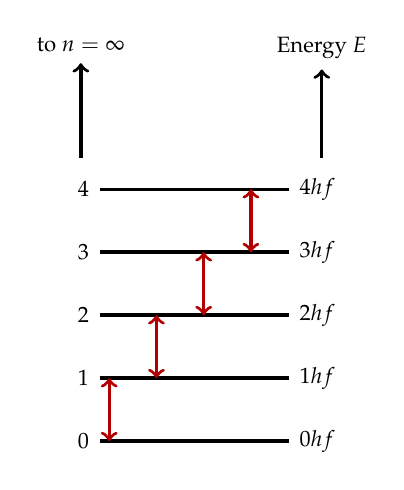
\begin{tikzpicture}[xscale=.6,yscale=.8]
      \foreach \y in {0,1,...,4} {
        \draw[very thick](0,\y)--(4,\y)
        node[pos=0,left] {\footnotesize $\y$}
        node[pos=1,right]{\footnotesize $\y hf$};
      }
      \foreach \y in {0,1,...,3} {
        \draw[very thick,red!70!black,<->](\y+.2,\y)--(\y+.2,\y+1);
      }
      \draw[very thick,->](4.7,4.5)--(4.7,5.9)
      node[pos=1,above]{\footnotesize Energy $E$};
      \draw[very thick,->](-.4,4.5)--(-.4,6)
      node[pos=1,above]{\footnotesize to $n=\infty$};
    \end{tikzpicture}
  \end{columns}
\end{frame}



\begin{frame}{Planck's Law}
  As for his formula, it's called \textbf{Planck's law}:

  \eq{-.01in}{
    \boxed{
      P(\lambda,T)=\frac{2hc^2}{\lambda^5}\frac{1}{e^{\frac{hc}{\lambda k_BT}}-1}
    }
  }
\end{frame}



\begin{frame}{Classical vs. Quantum Oscillator}
  This ``quantum'' behavior exists even for the simple pendulum that we studied
  in mechanics topics in harmonic motion and circular motion:
  \begin{columns}
    \column{.2\textwidth}
    \begin{tikzpicture}
      \fill[pattern=north east lines] (-1,0) rectangle (1,0.2);
      \draw[very thick](-1,0)--(1,0);
      \begin{scope}[rotate=10]
        \draw[thick](0,0)--(0,-5) node[midway,right]{$\ell$};
        \tikzstyle{balloon}=[ball color=red];    
        \shade[balloon] (0,-5) circle (0.2) node[below right]{$m$};
      \end{scope}
      \draw[dashed,thin](0,0)--(0,-5);
      \draw[->](0,-2) arc(270:280:2) node[pos=0.5,below]{$\theta$};
    \end{tikzpicture}

    \column{.78\textwidth}
    The natural frequency for $\ell=\SI{1}{\metre}$
    \begin{displaymath}
      \vspace{-.2in}
      f=\frac{1}{2\pi}\sqrt{\frac{g}{\ell}}\approx\SI{.50}{\hertz}
    \end{displaymath}
    \vspace{-.1in}Each energy level
    \begin{displaymath}
      \vspace{-.1in}
      \Delta E=hf\approx\SI{3.3e-34}{\joule}
    \end{displaymath}
    
    For a pendulum with $m=$\SI{100}{\gram} and $\theta=$\ang{10}:
    \begin{displaymath}
      \vspace{-.1in}
      \frac{\Delta E}{E}=\frac{\Delta E}{mg\ell(1-\cos\theta)}
      \approx\SI{2.2e-32}{\joule}
    \end{displaymath}
    No wonder we can't observe it in a marcoscopic level!
  \end{columns}
\end{frame}

\begin{frame}{Maxwell's Equations in a Vacuum}
  \vspace{-.1in}{\Large
    \begin{align*}
      \nabla\cdot\mb{E} &= 0\\
      \nabla\cdot\mb{B} &= 0\\
      \nabla\times\mb{E} &=-\frac{\partial\mb{B}}{\partial t}\\
      \nabla\times\mb{B} &=\mu_o\varepsilon_o\frac{\partial\mb{E}}{\partial t}
    \end{align*}
  }
  
  \vspace{-.15in}Disturbances in $\mb{E}$ and $\mb{B}$ travel as an
  ``electromagnetic wave'', with a speed:

  \eq{-.25in}{
    c=\frac{1}{\sqrt{\varepsilon_0\mu_0}}=\SI{299792458}{m/s}
  }
\end{frame}


\begin{frame}{The Spark Gap Experiment}
  To prove that light is an EM wave, German physicist Heinrich Hertz devised a
  ``spark gap experiment'' to generate frequencies in the range of
  \SI{e14}{\hertz}
  \begin{center}
    \pic{.55}{Hertz_exp_2.png}
  \end{center}
  \begin{itemize}
  \item\vspace{-.1in}Also showed that light has the same wavelengths as
    predicted by Maxwell's equations
  \item Discovered \textbf{photoelectric effect} that was caused by ultraviolet
    radiation
  \item Physicist who repeated his experiments did not have an explanation
  \end{itemize}
\end{frame}


\begin{frame}{Photoelectric Effect}
  When electromagnetic waves (e.g. light) hits certain metals, electrons are
  knocked off the surface.
  \begin{center}
    \pic{.9}{73bacc9f2bf571752483a89ef6c61a94f07470f7.png}
  \end{center}
  When observing this \textbf{photoelectric effect}, physicists discovered that:
  \begin{itemize}
  \item Increasing intensity of light knocked off more electrons, but doesn't
    change the maximum kinetic energy of the electrons, but
  \item Changing the frequency of the light did change $K$ though, although
  \item Below a certain frequency, \emph{no} electrons were emitted
  \end{itemize}
\end{frame}


\begin{frame}
  \frametitle{The Photon: Packets of Energy}
  In the 1905 paper \emph{On a Heuristic Viewpoint Concerning the Production and
    Transformation of Light}, Einstein argued that light is not continuous
  wave, but a collection of discrete energy packets (photons), each with energy
  $E=hf$

  \eq{-.22in}{
    \boxed{K_\mathrm{max}=
      \begin{cases}
        hf-\varphi & \text{if }hf>\varphi\\
        0          & \text{otherwise}
      \end{cases}
    }
  }
  \begin{center}
    \begin{tabular}{l|c|c}
      \rowcolor{pink}
      \textbf{Quantity} & \textbf{Symbol} & \textbf{SI Unit} \\ \hline
      Maximum kinetic energy of   & $K_\mathrm{max}$ & \si{\joule}\\
      Planck's constant           & $h$   & \si{\joule.\second}\\
      Frequency of the EM wave    & $f$   & \si{\hertz}\\
      Work function of the metal  & $\varphi$ & \si{\joule}
    \end{tabular}
  \end{center}
  Einstein may have been alerted to the fact that the blackbody radiation curve
  resembles the distribution of energies in a gas
\end{frame}



\begin{frame}{Work Function}
  \begin{columns}
  \column{.5\textwidth}
  \pic{1}{550px-Photoelectric_effect_diagram.png}
  
  \column{.5\textwidth}
  \textbf{Work function} the minimum energy required to remove an electron
  from a solid to a point immediately outside the solid surface. The minimum
  frequency at which electrons will be ejected is called the
  \textbf{threshold frequency}.

  \vspace{.15in}Slope is $h$ no matter what metal it is.
  \end{columns}
\end{frame}



\begin{frame}{Work Functions of Different Materials}
  The work function $\varphi$ depends on the metal. They are generally presented
  in electron volts.
  \begin{center}
    \pic{.35}{work-function.png}
  \end{center}
\end{frame}


\begin{frame}
  \frametitle{Compton Scattering}
  American physicist Arthur Holly Compton studied x-ray scattering by free
  electrons
  \begin{itemize}
  \item Classical theory cannot account for the scattering behaviour
  \item Frequency shift only depends on scattering angle
  \item Prediction possible if treating the x-ray as photons with
    momentum, just like a particle. Compton used Einstein's invariant and
    applied to a massless particle:
  \end{itemize}

  \eq{-.3in}{
    \boxed{p=\frac{E}{c}=\frac{hf}{c}=\frac{h}{\lambda}}
  }
\end{frame}

\begin{frame}
  \frametitle{Compton Scattering}
  \begin{center}
    \pic{.5}{compton2.png}
  \end{center}
  If we treat the x-ray as a photon with momentum $p=h/\lambda$ then we can
  use Newton's laws of motion to predict both the recoil electron and scattered
  x-ray!
\end{frame}

\begin{frame}
  \frametitle{Momentum of a Photon}
  The momentum of a photon is proportional to Planck's constant and 
  inversely proportional to its wavelength.

  \eq{-.2in}{
    \boxed{p=\frac{h}{\lambda}}
  }
  \begin{center}
    \begin{tabular}{l|c|c}
      \rowcolor{pink}
      \textbf{Quantity} & \textbf{Symbol} & \textbf{SI Unit} \\ \hline
      Momentum          & $p$ & \si{\kilo\gram.\metre/\second}\\
      Planck's constant & $h$ & \si{\joule.\second}\\
      Wavelength        & $\lambda$ & \si{\metre}
    \end{tabular}
  \end{center}
  This is a very odd expression, which treats photon both as a particle (with
  momentum) and a wave (with a wavelength $\lambda$).
\end{frame}

%\begin{frame}
%  \frametitle{Example Problem}
%  \textbf{Example 1}: Calculate the momentum of a photon of light that has
%  frequency of $5.09\e{14}\mathrm{Hz}$.
%\end{frame}



\begin{frame}{Matter Waves}
  If electromagnetic waves are really particles of energy, then are particles
  (e.g.\ electrons) a wave of some sort?
  \begin{itemize}
  \item The De Broglie hypothesis in 1924: a particle can also have a
    wavelength
  \item Confirmed accidentally by the Davisson-Germer Experiment in 1927 (beam
    of electron scattering on nickel crystal surface)
  \end{itemize}

  \vspace{.1in}If a particle is also a wave, what \emph{kind} of a wave is it
  then?
\end{frame}



\begin{frame}
  \frametitle{Electron Interference}
  \begin{columns}
    \column{.82\textwidth}
    If I perform a double-slit experiment with a beam of electrons, will I get
    an interference pattern?
    \begin{center}
      \pic{.7}{CNX_Chem_06_03_Electrnin.png}
    \end{center}

    \column{.18\textwidth}
    \pic{1}{206px-Double-slit_experiment_results_Tanamura_2.jpg}
  \end{columns}
\end{frame}



\begin{frame}
  \frametitle{De Broglie Wavelength}
  If matter is also a wave, then its wavelength can be obtained by solving the
  momentum equation for $\lambda$:

  \eq{-.2in}{
    p=\frac{h}{\lambda}\;\;\rightarrow\;\;
    \lambda=\frac{h}{p}\;\;\rightarrow\;\;\boxed{\lambda=\frac{h}{mv}}
  }

  \vspace{-.1in}
  \begin{center}
    \begin{tabular}{l|c|c}
      \rowcolor{pink}
      \textbf{Quantity} & \textbf{Symbol} & \textbf{SI Unit} \\ \hline
      Wavelength of a particle & $\lambda$ & \si{\metre} \\
      Planck's constant & $h$  & \si{\joule.\second} \\
      Mass              & $m$  & \si{\kilo\gram} \\
      Velocity          & $v$  & \si{\metre/\second}
    \end{tabular}
  \end{center}
\end{frame}



\begin{frame}{Uncertainty Principle}
  If a particle is a wave, how do you tell where it is?
  \begin{center}
    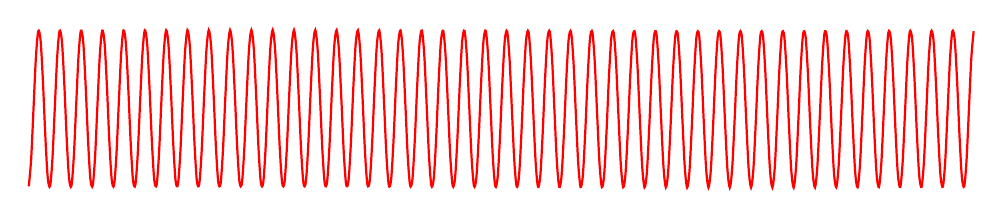
\begin{tikzpicture}

      \draw[xscale=.3,thick,red,smooth,samples=400,domain=-20:20]
      plot({\x},{sin(400*\x)});
    \end{tikzpicture}
    
    {\footnotesize $\cos(400x)$}
  \end{center}
  \begin{itemize}
  \item This wave/particle has a single wavelength $\lambda$ (therefore
    momentum $p$)
  \item Has no distinguishing features that can tell you its location $x$
  \item When we have precise knowledge of the particle wave's momentum (i.e.\
    its wavelength), then we have no idea where it is.
  \end{itemize} 
\end{frame}

\begin{frame}{Uncertainty Principle}
  Howeever, if a particle is defined as waves with small variations of
  wavelengths, when we add up the different waves together, we begin to see a
  \textbf{wave packet}:
  \begin{center}
    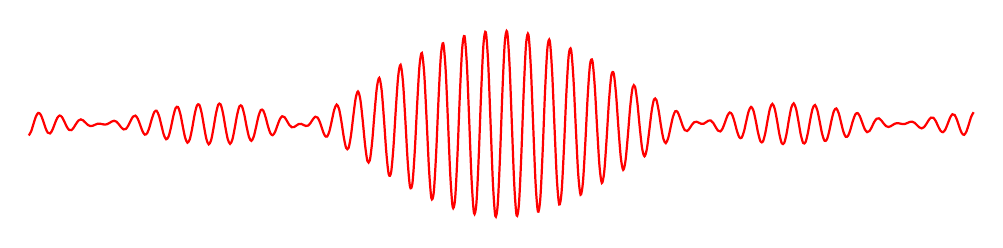
\begin{tikzpicture}
      \draw[xscale=.3,yscale=.07,thick,red,smooth,samples=400,domain=-20:20]
      plot({\x},{
        sin(400*\x)+
        sin(402.5*\x)+ sin(405*\x)+ sin(407.5*\x)+ sin(410*\x)+
        sin(412.5*\x)+ sin(415*\x)+ sin(417.5*\x)+ sin(420*\x)+
        sin(380*\x)+ sin(382.5*\x)+ sin(385*\x)+ sin(387.5*\x)+
        sin(390*\x)+ sin(392.5*\x)+ sin(395*\x)+ sin(397.5*\x)
      });
    \end{tikzpicture}

    {\footnotesize
      $\cos(380x)+\cos(382.5x)+\cdots+\cos(400x)+
      \cos(402.5x)+\cdots+\cos(420x)$}
  \end{center}
  Bottom line: In order to know more about the location of the particle, we
  \emph{must} lose information about its momentum.
\end{frame}


\begin{frame}{Heisenberg Uncertainty Principle}
  Because of the wave properties of particles, you can never be completely
  certain of the relationship between an object's momentum $p$ and position
  $x$. The more you know about an object's position, the less you know about
  its momentum, and vice versa.

  \eq{-.2in}{
    \boxed{\sigma_p\sigma_x\geq \frac{\hbar}{2}}
  }
  \begin{center}
    \begin{tabular}{l|c|c}
      \rowcolor{pink}
      \textbf{Quantity} & \textbf{Symbol} & \textbf{SI Unit} \\ \hline
      Uncertainty in momentum  & $\sigma_p$ & \si{\kilo\gram.\metre/\second}\\
      Uncertainty in position  & $\sigma_x$ & \si{\metre} \\
      Redued Planck's constant & $\hbar$    & \si{\joule\second}
    \end{tabular}
  \end{center}
  The \textbf{reduced Planck's constant} is just $\hbar=\frac{h}{2\pi}$.
\end{frame}




\begin{frame}{Bohr Atomic  Model}
  The ``orbital'' model of electrons does not work, because as the electron
  orbits (accelerates around) the nucleus, it radiates electromagnetic
  radiation, and therefore lose energy. The orbit will eventually collapse.

  \vspace{.1in} Bohr postulated that electron can move in certain
  ``non-radiating'' orbits, corresponding to energy levels:

  \eq{-.1in}{
    \boxed{E_n=-\frac{k^2e^4m}{2\hbar^2}\frac{Z^2}{n^2}}
  }
  
  From the wave-particle duality perspective, the ``orbits'' correspond more to
  a standing wave around the nucleus (a standing wave does not lose energy)
\end{frame}


\begin{frame}{Bohr Atomic Model}
  \eq{-.1in}{
    \boxed{E_n=-\frac{k^2e^4m}{2\hbar^2}\frac{Z^2}{n^2}}
  }
  \begin{center}
    \begin{tabular}{l|c|c}
      \rowcolor{pink}
      \textbf{Quantity} & \textbf{Symbol} & \textbf{SI Unit} \\ \hline
      Energy at level $n$ & $E_n$ & \si{\joule} \\
      Coulomb's constant & $k$ & \si{N.m^2/C^2} \\
      Elementary charge  & $e$ & \si{\coulomb} \\
      Atomic mass        & $m$ & \si{\kilo\gram} \\
      Reduced Planck's constant & $\hbar$ & \si{\joule.\second}\\
      Atomic number      & $Z$ & integer; no units\\
      Energy level       & $n$ & integer; no units
    \end{tabular}
  \end{center}
\end{frame}


\begin{frame}{Bohr Atomic  Model}
  Successful in describing the behaviour of the hydrogen atom---but fails for
  heavier atoms---although it still relies on 
  \begin{itemize}
  \item Coulomb forces between electrons and protons (classical)
  \item Centripetal forces (classical)
  \item Quantization of energy (new physics!)
  \end{itemize}
  De Broglie's hypothesis gives us a glimpse of what Bohr is missing
  \begin{itemize}
  \item The ``orbits'' correspond to a standing wave around the nucleus
  \item A standing wave does not lose energy
  \end{itemize}
\end{frame}


\begin{frame}{Hydrogen Emission}
  \begin{columns}

    \column{.6\textwidth}
    \begin{itemize}
    \item Lyman series:
      \begin{itemize}
      \item the EM emissions when the electrons drop from a higher energy state
        ($E_n$) to the ground state $n=1$ (i.e.\ $E_1$)
      \item The frequency is given by:
        
        \eq{-.2in}{
          f=\frac{E_1-E_n}{h}
        }
      \item We can apply universal wave equation to get the wavelengths
      \end{itemize}
    \item Balmer series--dropping to $E_2$
    \item Paschen series--dropping to $E_3$
    \end{itemize}

    \column{.4\textwidth}
    \pic{1}{400px-Hydrogen_transitions.png}
  \end{columns}
\end{frame}


\begin{frame}
  \frametitle{Standing Wave on a String}
  \begin{columns}
    \column{.3\textwidth}
    \pic{1}{strhar.png}

    \column{.7\textwidth}
    \begin{itemize}
    \item We have studied standing waves in Grade 11
    \item If electron is to be in a ``stable orbit'' around a nucleus, it has
      to be in a standing wave pattern
    \item Otherwise, it will interfere with itself
    \end{itemize}
  \end{columns}
\end{frame}


\begin{frame}
  \frametitle{Circular Standing Wave}
  \begin{center}
    \pic{.7}{oo1wp.png}
  \end{center}
  Electron resonance states $n=3,4,5,6$
\end{frame}



\begin{frame}
  \frametitle{Particle in a Box}
  \begin{columns}
    \column{.3\textwidth}
    \pic{1}{box.png}
    
    \column{.7\textwidth}
    A particle in a 1D box has to behave like a standing wave. The resonance
    modes (frequencies where a stable standing wave exists) correspond to the
    wavelengths:
    
    \eq{-.2in}{
      \lambda=\frac{2L}{n}\quad n=1,2,3,4,\ldots
    }
    and the momentum of the particle is:

    \eq{-.2in}{
      p=\frac{h}{\lambda}=\frac{nh}{2L}
    }
  \end{columns}
\end{frame}



\begin{frame}{Particle in a Box}
  \begin{columns}
    \column{.3\textwidth}
    \pic{1}{box.png}
    
    \column{.7\textwidth}
    Kinetic energy of the particle can be expressed in terms of momentum:

    \eq{-.2in}{
      K_n=\frac{1}{2}mv^2=\frac{p^2}{2m}=\frac{n^2h^2}{8mL^2}
    }

    If a particle is a standing wave, then kinetic energy of the particle can
    never be zero (as long as it is confined inside the box), therefore
    \begin{itemize}
    \item It cannot have zero velocity
    \item The lowest energy level ($n=1$) is called the
      \textbf{zero-point energy}
    \end{itemize}
  \end{columns}
\end{frame}


\begin{frame}
  \frametitle{Example}
  \textbf{Example 3:} A \SI{.150}{\kilo\gram} billiard ball is confined to the
  pool table \SI{1.42}{\metre} wide. How long (in seconds) will it take to
  travel from one side of the table to the other? (Use fundamental mode.)
\end{frame}

\end{document}
